\documentclass[11pt]{article}

\usepackage[letterpaper,margin=0.75in]{geometry}
\usepackage{booktabs}
\usepackage{graphicx}
\usepackage{listings}

\setlength{\parindent}{1.4em}

\newcommand{\code}[1]{\texttt{#1}}

\begin{document}

\lstset{
  language=Python,
  basicstyle=\small,          % print whole listing small
  keywordstyle=\bfseries,
  identifierstyle=,           % nothing happens
  commentstyle=,              % white comments
  stringstyle=\ttfamily,      % typewriter type for strings
  showstringspaces=false,     % no special string spaces
  numbers=left,
  numberstyle=\tiny,
  numbersep=5pt,
  frame=tb,
}

\title{Lab 4 Report}

\author{Nate Fox}

\date{}

\maketitle

\section{Congestion Control}

\subsection{Class Variables}
To implement congestion control, I started by changing some of the TCP class variables. I renamed the \code{window} variable to \code{cwnd} in order to match the variable names from the textbook, and I initialized \code{cwnd} to be one MSS. I also introduced the \code{ssthresh} variable to keep track of the slow start threshold. Finally I introduced the \code{ack\_count} variable to keep track of duplicate ACKs.

\subsection{Receiving New ACKs}
When I receive ACKs for newly acknowledged data, I update my congestion window according to what state I am in. If my current \code{cwnd} is less than \code{ssthresh}, I consider myself in slow start mode and I increment \code{cwnd} by the number of new bytes acknowledged. If my current \code{cwnd} is greater than or equal to \code{ssthresh}, I consider myself in AIMD mode and I increment \code{cwnd} by (MSS * new\_bytes / \code{cwnd}). I also reset my \code{ack\_count} to 0.
 
\subsection{Receiving Duplicate ACKs}
When I receive a duplicate ACK, I increment my \code{ack\_count}. If \code{ack\_count} is three after I increment it, I retransmit without restarting the retransmission timer or updating the RTO.

\subsection{Retransmitting}
Whenever I retransmit, either due to the retransmission timer firing or due to three duplicate ACKs, I update the \code{ssthresh} and the \code{cwnd}. I set \code{ssthresh} to one-half of \code{cwnd} (to a minimum of one MSS) and I reset \code{cwnd} to one MSS.

\section{Basic Experiments}

\subsection{Setup}
The network consists of two nodes with a single bidirectional link between them. The link has a 1 Mbps bandwidth and a propagation delay of 10ms. The queue size is limited to 20 packets (20,000 bytes). The initial \code{ssthresh} is set to 100,000 bytes.

\pagebreak
\subsection{One Flow}
With the aforementioned setup, a 1 MB file is transmitted over the link.

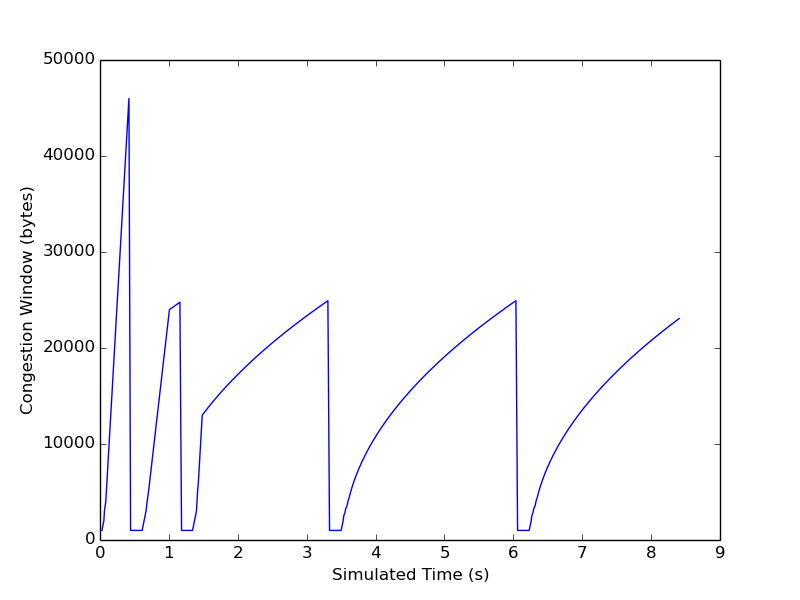
\includegraphics[width=10cm]{../graphs/one_flow_cwnd.png}

The above graph shows the typical sawtooth pattern as the congestion window reacts to the congestion of the network. When a packet is dropped, the congestion window updates \code{ssthresh} and resets to 1,000 bytes. The congestion window grows exponentially in slow start mode until \code{ssthresh} is reached, at which point additive increase begins.

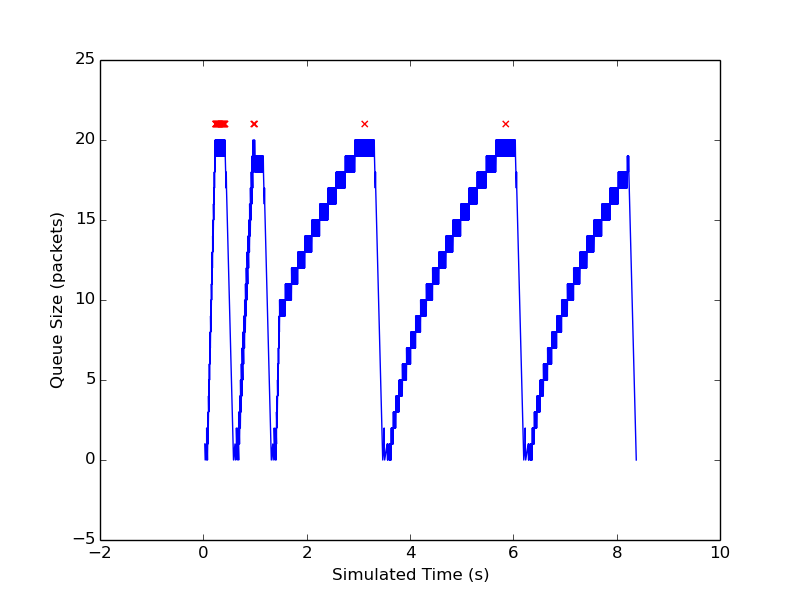
\includegraphics[width=10cm]{../graphs/one_flow_queue_size.png}

The above graph shows how the queue size changes over time. When packets are dropped due to queue overflow (marked by red X), the sender resets the congestion window to 1,000 bytes, which lessens the stress on the queue. For this reason, the queue size graph is comparable to the congestion window graph.

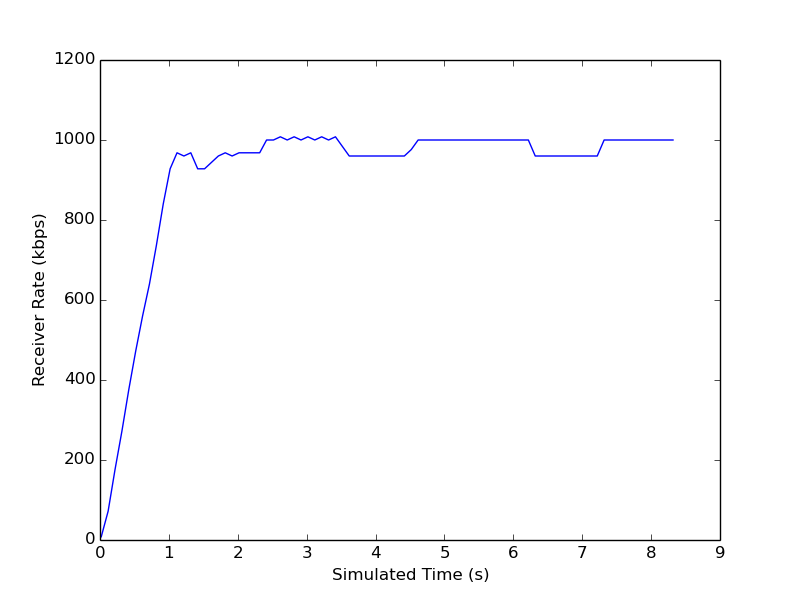
\includegraphics[width=10cm]{../graphs/one_flow_receiver_rate.png}

As shown in the above graph, the receive rate rapidly increases and then levels out at the full link bandwidth.

\subsection{Two Flows}
I wrote a new python script \code{two\_flow.py} and a new shell script \code{run\_two\_flow.sh} to send two flows over a single link in parallel. I modified log messages from \code{tcp.py} to include information on which flow the log messages pertained to. I also modified \code{plot.py} to graph separate lines for each flow on the receive rate and congestion window graphs. A 1 MB file is transmitted over each flow on the link.

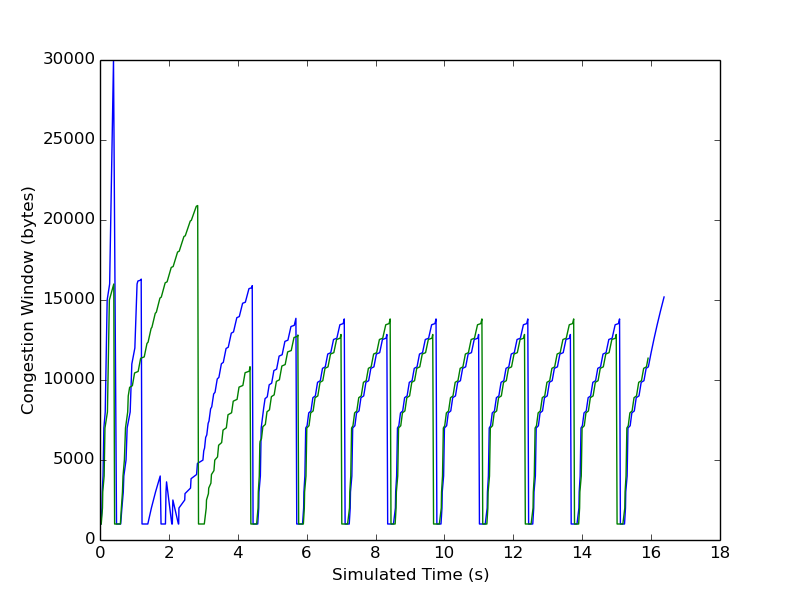
\includegraphics[width=10cm]{../graphs/two_flow_cwnd.png}

The congestion window graph above shows that both flows experienced the typical sawtooth pattern. They start out differently, but after a few seconds they adjust and follow the same pattern.

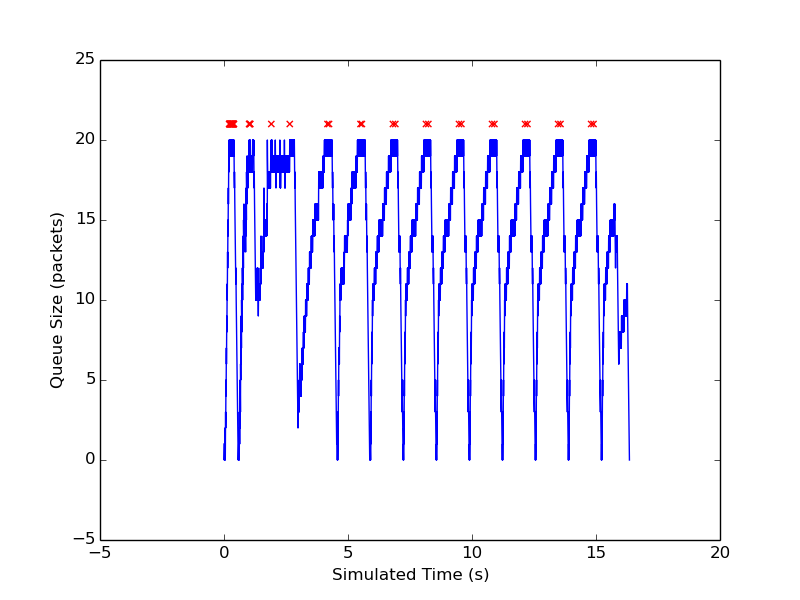
\includegraphics[width=10cm]{../graphs/two_flow_queue_size.png}

With two flows over the same link, the queue overflows a lot more. The queue graph still looks very similar to the congestion window graph, particularly after a few seconds when both flows' congestion windows follow the same pattern.

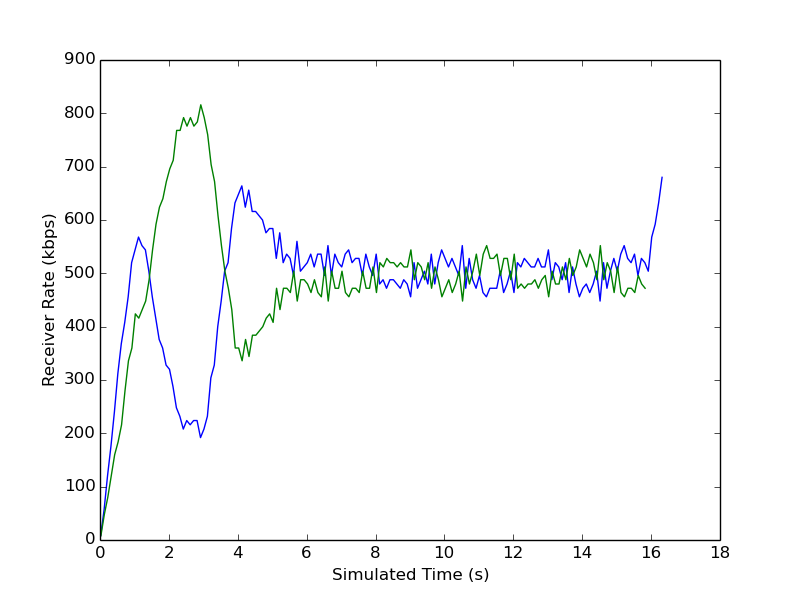
\includegraphics[width=10cm]{../graphs/two_flow_receiver_rate.png}

The first flow (blue line), detected packet loss before the second flow (green line), so the first flow drops to about 200 kbps and the second flow jumps up to use the remaining 800 kbps. Over time, the two flows converge around 500 kbps, which is half the link bandwidth. The file transfer finishes slightly earlier on the second flow, allowing the first flow to use more bandwidth as it finishes the transfer.

\subsection{Five Flows}
I wrote a new python script \code{five\_flow.py} and a new shell script \code{run\_five\_flow.sh} to send five flows over a single link in parallel. A 1 MB file is transmitted over each flow on the link, with a 1.5 second offset between each flow.

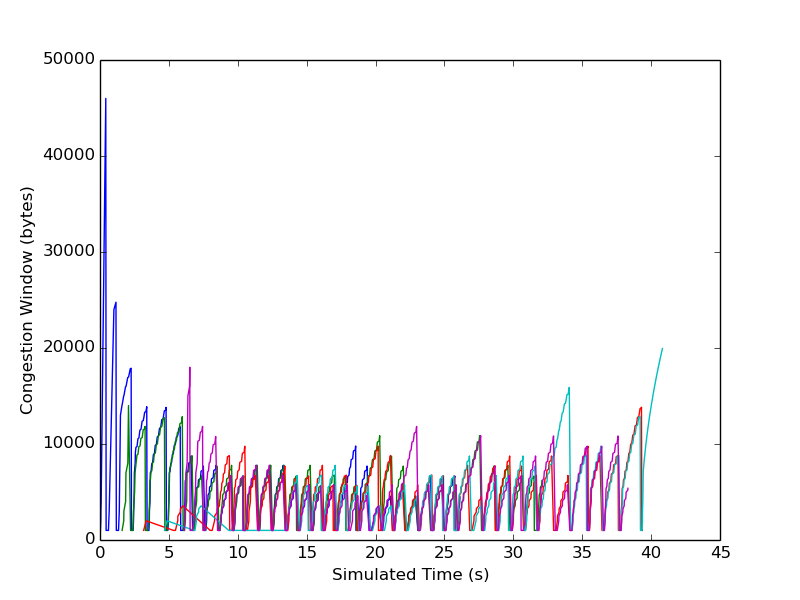
\includegraphics[width=10cm]{../graphs/five_flow_cwnd.png}

The above graph shows a very condensed sawtooth pattern. With five separate flows each transferring a 1 MB file over a link with a queue that only holds 20 packets, packet loss occurs frequently, resulting in a low \code{ssthresh} and frequent \code{cwnd} resets.

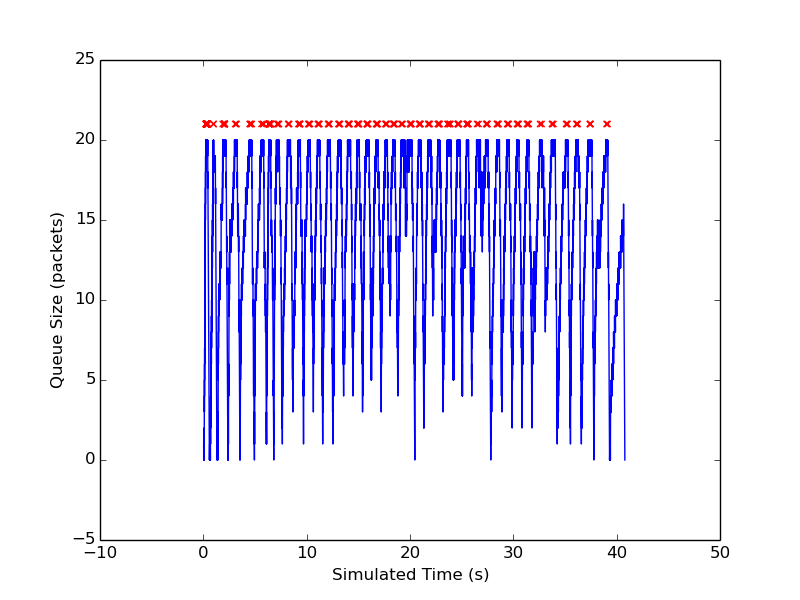
\includegraphics[width=10cm]{../graphs/five_flow_queue_size.png}

As previously discussed, packet loss occurs frequently with such a high load.

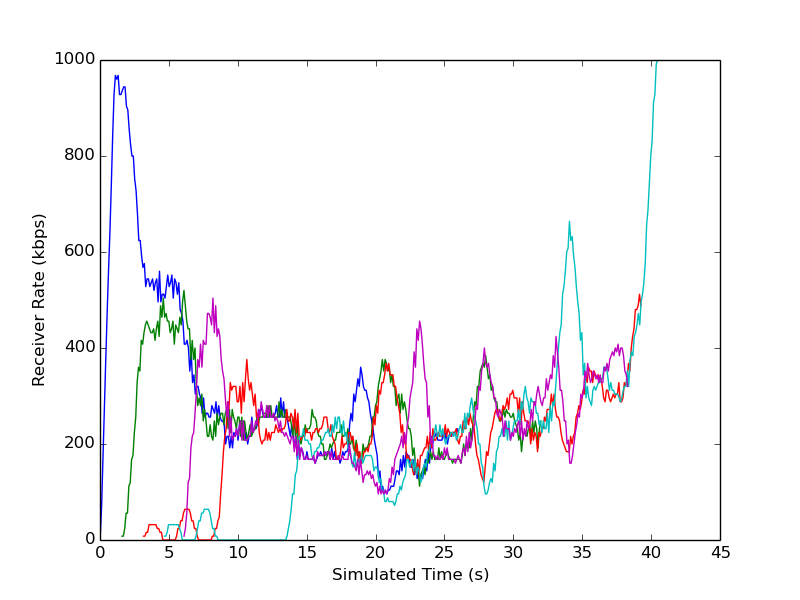
\includegraphics[width=10cm]{../graphs/five_flow_receiver_rate.png}

The 1.5 second offset between flows lets the first flow (blue line) use the full bandwidth for a short time. When the second flow (green line) comes in, the two flows adjust to about 500 kbps each. Once all five flows come in, they all eventually adjust to 100-300 kbps each until the first flow finishes the file transfer. The remaining flows use the extra bandwidth, and at the end there is a single flow that gets all the bandwidth to finish its file transfer.

\section{Advanced Experiments}

\subsection{AIAD}
I changed my \code{tcp.py} code to use AIAD rather than AIMD:
\begin{lstlisting}
def do_retransmit(self):
	# Set ssthresh and cwnd
	#self.ssthresh = max(self.cwnd/2, self.mss)
	self.ssthresh = max(self.ssthresh-self.mss, self.mss)
	self.cwnd = self.mss
\end{lstlisting}
With the same network setup described in the previous section, I sent a 1 MB file over a single flow.

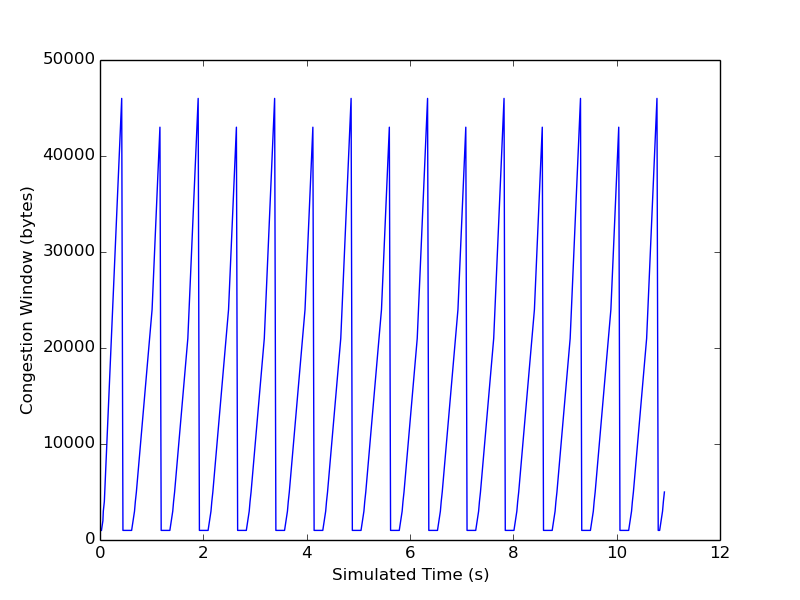
\includegraphics[width=10cm]{../graphs/aiad_cwnd.png}

With AIAD, the congestion window does not follow the familiar sawtooth pattern. Instead, it quickly oscillates back and forth with no evidence that it will ever converge.

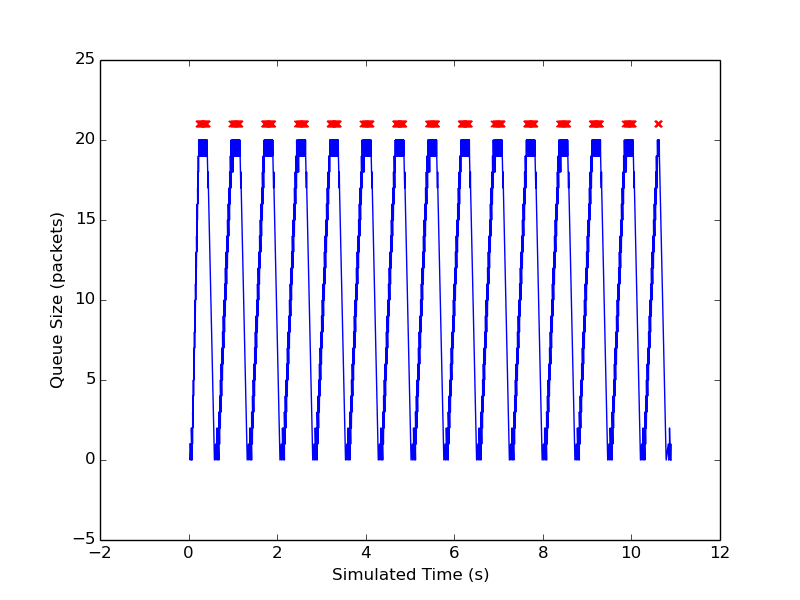
\includegraphics[width=10cm]{../graphs/aiad_queue_size.png}

Since the congestion window osciallates back and forth so quickly, the queue is frequently overwhelmed. With AIMD only a few packets were dropped, but many packets are dropped with AIAD.

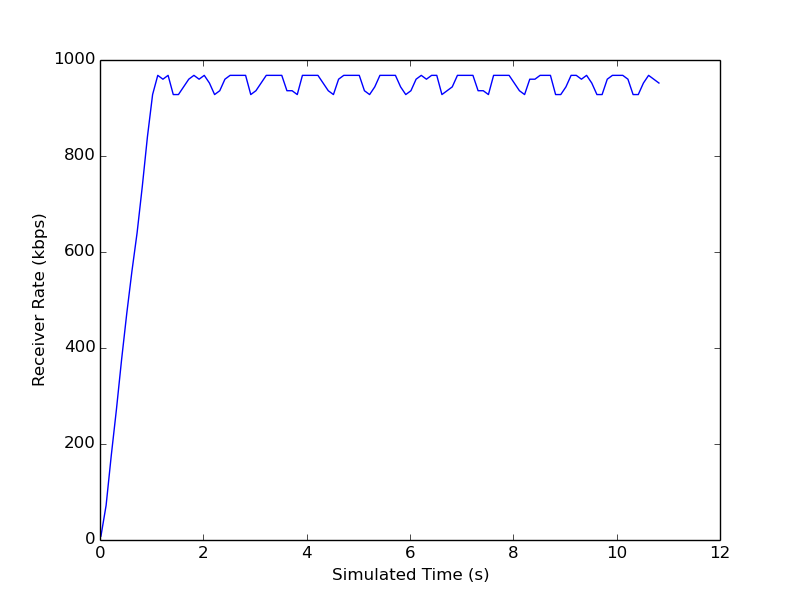
\includegraphics[width=10cm]{../graphs/aiad_receiver_rate.png}

As shown in the above graph, AIAD never allows the single flow to use the full 1 Mbps bandwidth. Instead, the bandwidth oscillates between 928 and 968 kbps with no evidence that it will ever converge.

When AIAD is used instead of AIMD, TCP ceases to show stable behavior. The bandwidth is not fully utilised, and the congestion window does not really help to prevent network congestion.

\pagebreak
\subsection{AIMD - Different Multiplicative Constant}
I changed my \code{tcp.py} code to use AIAD with a multiplicative constant of 5/6 instead of 1/2:
\begin{lstlisting}
def do_retransmit(self):
	# Set ssthresh and cwnd
	#self.ssthresh = max(self.cwnd/2, self.mss)
	self.ssthresh = max(self.cwnd * 5 / 6, self.mss)
	self.cwnd = self.mss
\end{lstlisting}

I sent a 1MB file over a single flow.

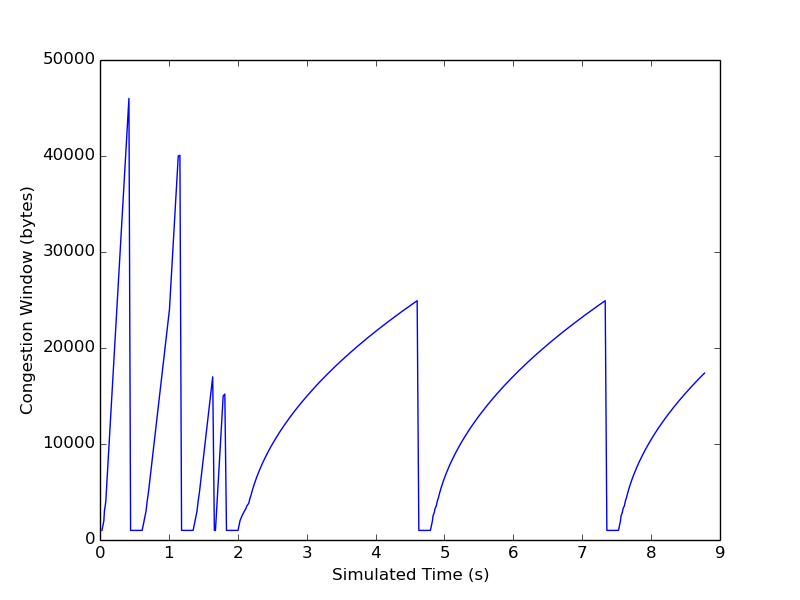
\includegraphics[width=10cm]{../graphs/aimdconst_cwnd.png}

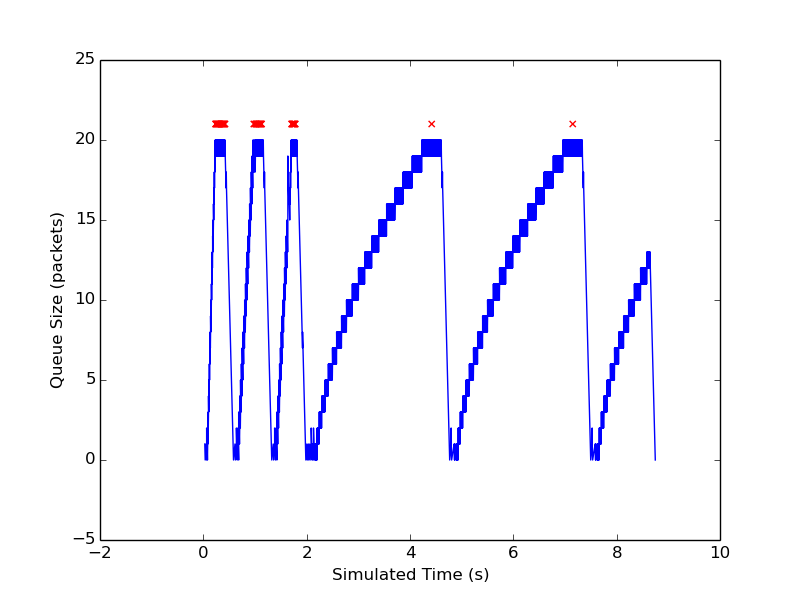
\includegraphics[width=10cm]{../graphs/aimdconst_queue_size.png}

With a multiplicative constant of 1/2, the congestion window started showing the familiar sawtooth pattern after about 1 second. With the new constant of 5/6, the congestion window takes a little longer before starting the sawtooth pattern. As shown in the Queue Size graph above, this leads to more packet loss in the first 2 seconds, but it does start to regulate itself better after that.

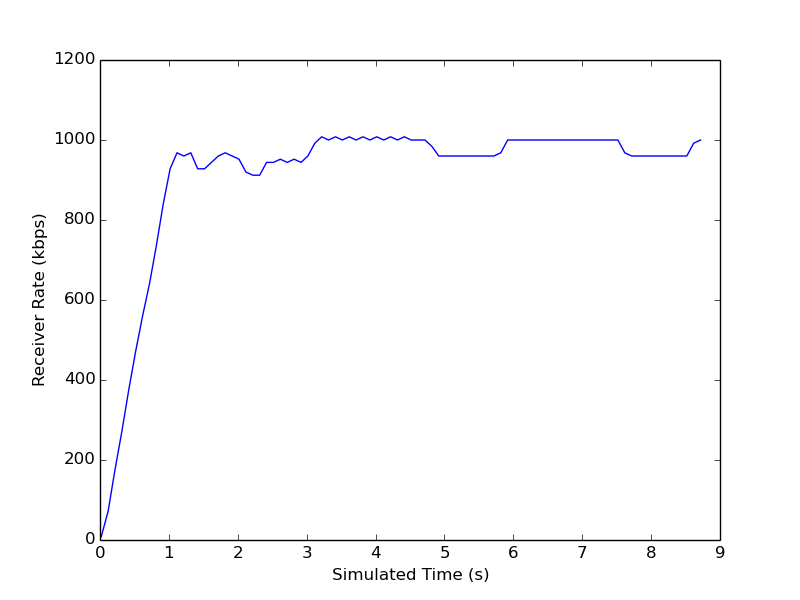
\includegraphics[width=10cm]{../graphs/aimdconst_receiver_rate.png}

With a multiplicative constant of 5/6, it takes the flow a little longer before it uses the full bandwidth amount, but it does get there eventually. Using a multiplicative constant of 5/6 causes the transfer time to be about 12\% longer than the transfer time is with a multiplicative constant of 1/2.

When a different multiplicative constant is used, TCP still shows stable behavior, though for this particular case it seems that 1/2 is a better constant than 5/6 is.

\subsection{Competing AIMD}
I changed my \code{tcp.py} code to use different multiplicative constants for a two-flow scenario:
\begin{lstlisting}
def do_retransmit(self):
	# Set ssthresh and cwnd
	if self.source_port == 1:
		self.ssthresh = max(self.cwnd/2, self.mss)
	else:
		self.ssthresh = max(self.cwnd * 5 / 6, self.mss)
	self.cwnd = self.mss
\end{lstlisting}
A 1 MB file is sent over both flows.

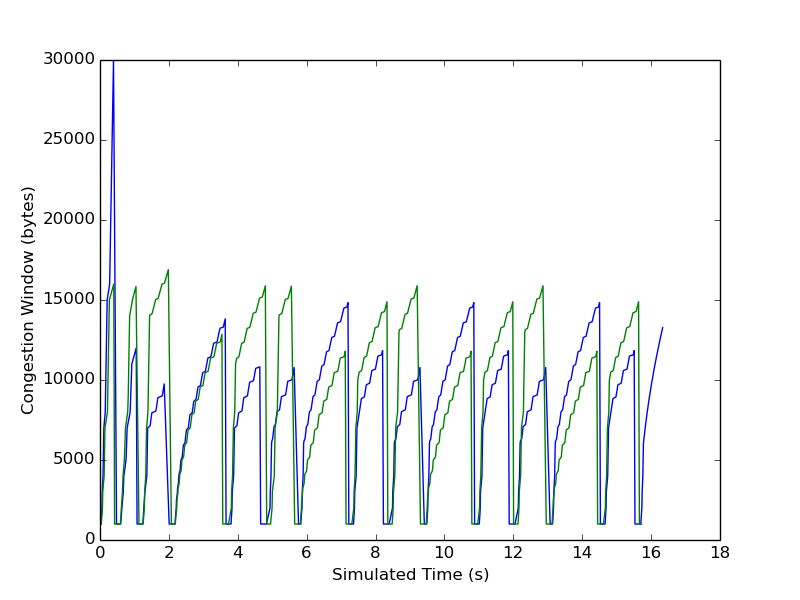
\includegraphics[width=10cm]{../graphs/aimdcompt_cwnd.png}

When both flows had the same multiplicative constant of 1/2, they eventually got to the point where their congestion windows overlapped almost perfectly. In this case, the second flow (green line) with a constant of 5/6 usually has a larger congestion window than the first flow does.

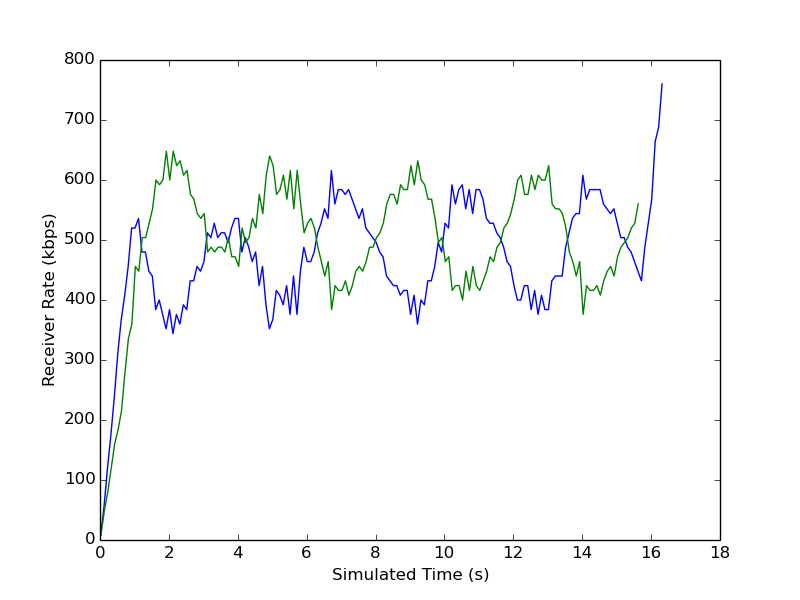
\includegraphics[width=10cm]{../graphs/aimdcompt_receiver_rate.png}

Both flows still seem to get their fair share of the bandwidth, but it is different from the case where both flows use a constant of 1/2. In the first case, both flows seemed to oscillate back and forth between 450 and 550 kbps. In the second case, the flows seem to oscillate back and forth between 350 and 650 kbps. In both cases, each flow averages about 500 kbps for the file transfer, but in the second case the distance from the average is more extreme for each flow.

\subsection{Competing RTT}

I created a new network, \code{split-network.txt}, which is set up like this:
\begin{lstlisting}
# n1
#  \
#   n3 -- n4
#  /
# n2
n1 n3
n2 n3
n3 n1 n2 n4
n4 n3

# link configuration
n1 n3 1Mbps 100ms
n3 n1 1Mbps 100ms
n2 n3 1Mbps 10ms
n3 n2 1Mbps 10ms
n3 n4 1Mbps 10ms
n4 n3 1Mbps 10ms
\end{lstlisting}

I wrote a new python script \code{compete\_rtt.py} and a new bash script \code{run\_compete\_rtt.sh} that use \code{split-network}. One flow is routed betwen n1 and n4, the other between n2 and n4. I send a 1 MB file over each flow, starting at the same time.

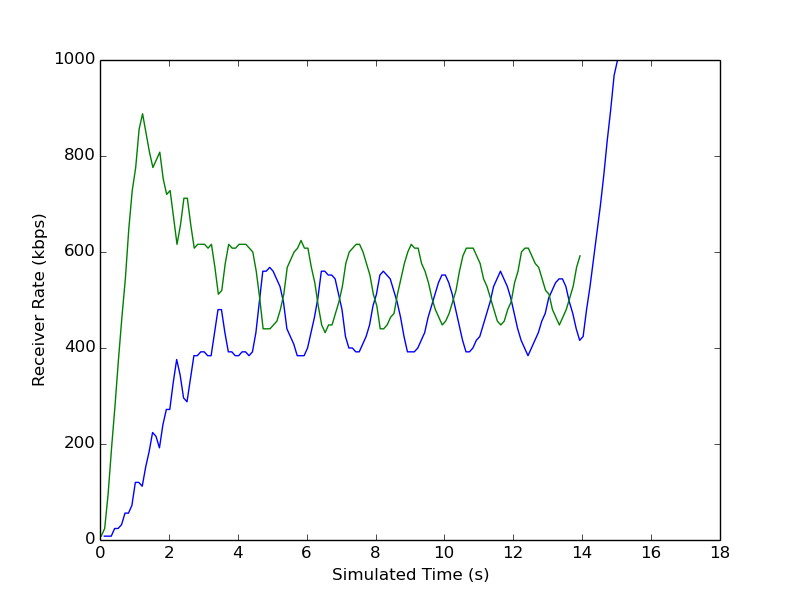
\includegraphics[width=10cm]{../graphs/compete_receiver_rate.png}

The first flow (blue line) has a longer propagation delay on its first link than the second flow (green line) has on its first link. The first flow's \code{cwnd} does not grow as fast because the round trip time is longer, and the \code{cwnd} only grows when it receives ACKs. Due to this, the first flow starts off slower and the second flow uses more bandwidth. Once the first flow catches up, the two oscillate back and forth around the equal share line. Each flow still gets its fair share of bandwidth.

\end{document}
